%{\color{red} This will get longer, with a result}.
Sometimes we are given a
high-rank embedding (resulting from h-MDS, for example), and wish to
find a lower-rank version.
In Euclidean space, one can get the optimal
lower rank embedding by simply discarding components. However, this
may not be the case in hyperbolic space.
Motivated by this, we study dimensionality reduction in hyperbolic space.

As hyperbolic space does not have a linear subspace structure like
Euclidean space, we need to define what we mean by lower-dimensional.
We follow Principal Geodesic Analysis~\cite{PGA}, \cite{GPCA}. Consider an initial
embedding with points $x_1,\dots,x_n \in \mathbb{H}_2$ and let $d_{H}
: \mathbb{H}_2 \times \mathbb{H}_2 \to \mathbb{R}_{+}$ be the hyperbolic distance.
Suppose we want to map this embedding onto a one-dimensional subspace. (Note that
we are considering a two-dimensional embedding and one-dimensional subspace
here for simplicity, and these
results immediately extend to higher dimensions.) In this case, the goal of PGA
is to find a geodesic $\gamma :
[0,1] \to \mathbb{H}_2$ that passes through the mean of the points and that minimizes the squared error (or variance):
\[ f(\gamma) = \sum_{i=1}^n \min_{t \in [0,1]} d_{H}(\gamma(t),x_i)^2 .\]
This expression can be simplified significantly and reduced to a
minimization in Euclidean space.  First, we find the mean of the
points, the point $\bar x$ which minimizes $\sum_{i=1}^n d_{H}(\bar
x, x_i)^2$; this definition in terms of distances generalizes the mean in Euclidean space.\footnote{As we noted earlier, considering the distances
without squares leads to a non-continuously-differentiable
formulation.}  Next, we reflect all the points $x_i$ so that their
mean is $0$ in the Poincar{\'e} disk model; we can do this using a
circle inversion that maps $\bar x$ onto $0$.
In the Poincar{\'e} disk model, a geodesic through
the origin is a Euclidean line, and the action of the reflection across
this line is the same in both Euclidean and hyperbolic space. Coupled
with the fact that reflections are isometric, if $\gamma$ is a line
through $0$ and $R_\gamma$ is the reflection across $\gamma$, we have
\[
  d_H(\gamma, x) = \min_{t \in [0,1]} d_H(\gamma(t), x) = \frac{1}{2} d_H(R_l x, x).
\]
Combining this with the Euclidean reflection formula and the hyperbolic metric produces
\[
  f(\gamma) = \frac{1}{4} \sum_{i=1}^n \acosh^2\left( 1 + \frac{ 8 d_{E}(\gamma,x_i)^2 }{(1 - \| x_i \|^2)^2} \right),
\]
in which $d_{E}$ is the Euclidean distance from a point to a line. If
we define $w_i = \sqrt{8} x_i / (1 - \| x_i \|^2)$ this reduces to the simplified expression
\[
  f(\gamma) = \frac{1}{4} \sum_{i=1}^n \acosh^2\left( 1 + d_{E}(\gamma,w_i)^2 \right).
\]
  
Notice that \emph{the loss function is not convex}. We observe that
there can be multiple local minima that are attractive and stable, in
contrast to PCA.  Figure~\ref{fig:pga} illustrates this nonconvexity
on a simple dataset in $\mathbb{H}_2$ with only four examples.  This
makes globally optimizing the objective difficult.
\begin{figure}
\centering
\resizebox{0.48\textwidth}{!}{\large% GNUPLOT: LaTeX picture with Postscript
\begingroup
  \makeatletter
  \providecommand\color[2][]{%
    \GenericError{(gnuplot) \space\space\space\@spaces}{%
      Package color not loaded in conjunction with
      terminal option `colourtext'%
    }{See the gnuplot documentation for explanation.%
    }{Either use 'blacktext' in gnuplot or load the package
      color.sty in LaTeX.}%
    \renewcommand\color[2][]{}%
  }%
  \providecommand\includegraphics[2][]{%
    \GenericError{(gnuplot) \space\space\space\@spaces}{%
      Package graphicx or graphics not loaded%
    }{See the gnuplot documentation for explanation.%
    }{The gnuplot epslatex terminal needs graphicx.sty or graphics.sty.}%
    \renewcommand\includegraphics[2][]{}%
  }%
  \providecommand\rotatebox[2]{#2}%
  \@ifundefined{ifGPcolor}{%
    \newif\ifGPcolor
    \GPcolortrue
  }{}%
  \@ifundefined{ifGPblacktext}{%
    \newif\ifGPblacktext
    \GPblacktextfalse
  }{}%
  % define a \g@addto@macro without @ in the name:
  \let\gplgaddtomacro\g@addto@macro
  % define empty templates for all commands taking text:
  \gdef\gplbacktext{}%
  \gdef\gplfronttext{}%
  \makeatother
  \ifGPblacktext
    % no textcolor at all
    \def\colorrgb#1{}%
    \def\colorgray#1{}%
  \else
    % gray or color?
    \ifGPcolor
      \def\colorrgb#1{\color[rgb]{#1}}%
      \def\colorgray#1{\color[gray]{#1}}%
      \expandafter\def\csname LTw\endcsname{\color{white}}%
      \expandafter\def\csname LTb\endcsname{\color{black}}%
      \expandafter\def\csname LTa\endcsname{\color{black}}%
      \expandafter\def\csname LT0\endcsname{\color[rgb]{1,0,0}}%
      \expandafter\def\csname LT1\endcsname{\color[rgb]{0,1,0}}%
      \expandafter\def\csname LT2\endcsname{\color[rgb]{0,0,1}}%
      \expandafter\def\csname LT3\endcsname{\color[rgb]{1,0,1}}%
      \expandafter\def\csname LT4\endcsname{\color[rgb]{0,1,1}}%
      \expandafter\def\csname LT5\endcsname{\color[rgb]{1,1,0}}%
      \expandafter\def\csname LT6\endcsname{\color[rgb]{0,0,0}}%
      \expandafter\def\csname LT7\endcsname{\color[rgb]{1,0.3,0}}%
      \expandafter\def\csname LT8\endcsname{\color[rgb]{0.5,0.5,0.5}}%
    \else
      % gray
      \def\colorrgb#1{\color{black}}%
      \def\colorgray#1{\color[gray]{#1}}%
      \expandafter\def\csname LTw\endcsname{\color{white}}%
      \expandafter\def\csname LTb\endcsname{\color{black}}%
      \expandafter\def\csname LTa\endcsname{\color{black}}%
      \expandafter\def\csname LT0\endcsname{\color{black}}%
      \expandafter\def\csname LT1\endcsname{\color{black}}%
      \expandafter\def\csname LT2\endcsname{\color{black}}%
      \expandafter\def\csname LT3\endcsname{\color{black}}%
      \expandafter\def\csname LT4\endcsname{\color{black}}%
      \expandafter\def\csname LT5\endcsname{\color{black}}%
      \expandafter\def\csname LT6\endcsname{\color{black}}%
      \expandafter\def\csname LT7\endcsname{\color{black}}%
      \expandafter\def\csname LT8\endcsname{\color{black}}%
    \fi
  \fi
    \setlength{\unitlength}{0.0500bp}%
    \ifx\gptboxheight\undefined%
      \newlength{\gptboxheight}%
      \newlength{\gptboxwidth}%
      \newsavebox{\gptboxtext}%
    \fi%
    \setlength{\fboxrule}{0.5pt}%
    \setlength{\fboxsep}{1pt}%
\begin{picture}(7200.00,3960.00)%
    \gplgaddtomacro\gplbacktext{%
      \csname LTb\endcsname%
      \put(682,704){\makebox(0,0)[r]{\strut{}$5$}}%
      \put(682,1131){\makebox(0,0)[r]{\strut{}$6$}}%
      \put(682,1559){\makebox(0,0)[r]{\strut{}$7$}}%
      \put(682,1986){\makebox(0,0)[r]{\strut{}$8$}}%
      \put(682,2413){\makebox(0,0)[r]{\strut{}$9$}}%
      \put(682,2840){\makebox(0,0)[r]{\strut{}$10$}}%
      \put(682,3268){\makebox(0,0)[r]{\strut{}$11$}}%
      \put(682,3695){\makebox(0,0)[r]{\strut{}$12$}}%
      \put(1428,484){\makebox(0,0){\strut{}0}}%
      \put(2634,484){\makebox(0,0){\strut{}$\pi/2$}}%
      \put(3840,484){\makebox(0,0){\strut{}$\pi$}}%
      \put(5047,484){\makebox(0,0){\strut{}$3\pi/2$}}%
      \put(6253,484){\makebox(0,0){\strut{}2$\pi$}}%
      \put(3885,918){\makebox(0,0)[l]{\strut{}non-global minima}}%
    }%
    \gplgaddtomacro\gplfronttext{%
      \csname LTb\endcsname%
      \put(176,2199){\rotatebox{-270}{\makebox(0,0){\strut{}PGA loss $f(\gamma)$}}}%
      \put(3808,154){\makebox(0,0){\strut{}angle of geodesic $\gamma$}}%
      \csname LTb\endcsname%
      \put(6344,3522){\makebox(0,0)[r]{\strut{}global minima}}%
    }%
    \gplbacktext
    \put(0,0){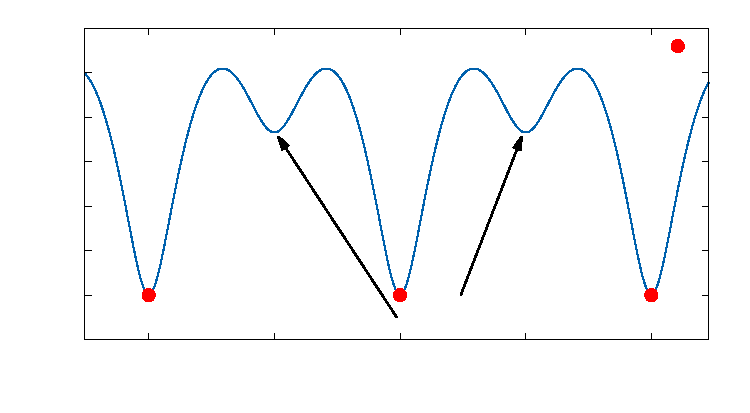
\includegraphics{gp/plotpga-eps-converted-to.pdf}}%
    \gplfronttext
  \end{picture}%
\endgroup
}
%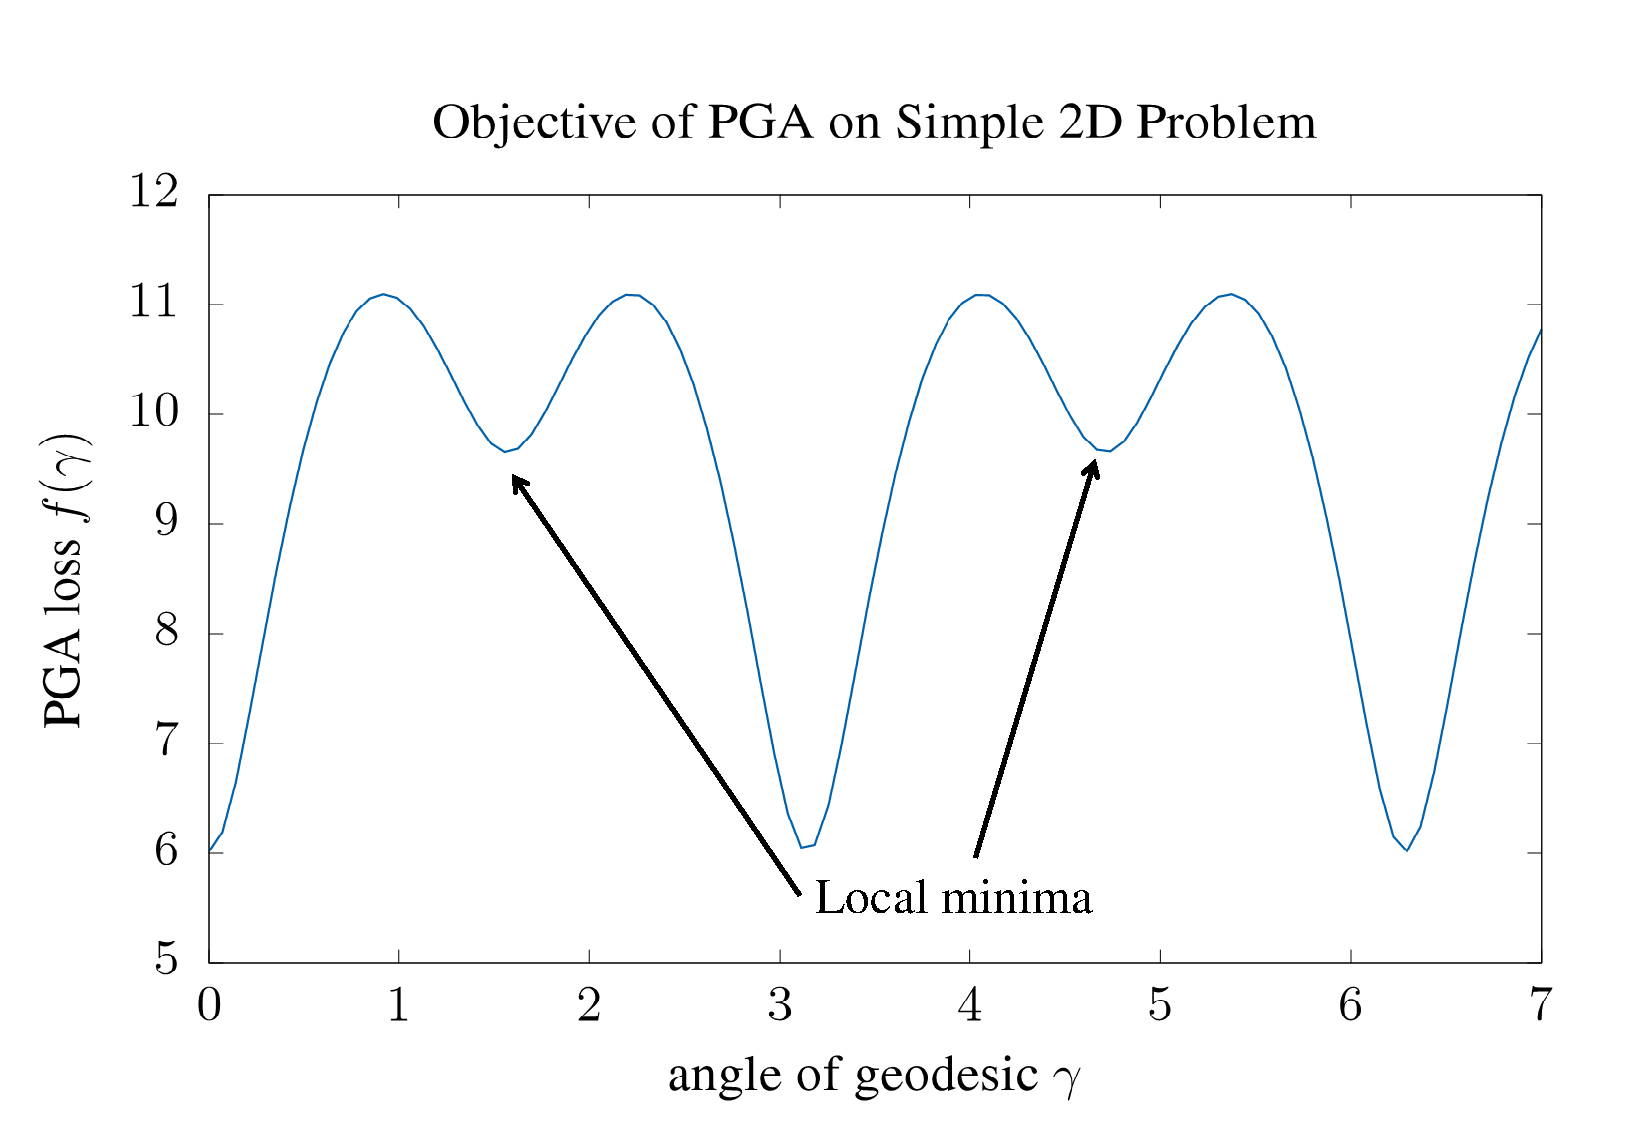
\includegraphics[width=0.3\textwidth]{gp/plotpga-labeled}
\caption{The PGA objective of an example task where the input dataset in the Poincar{\'e} disk is $x_1 = (0.8,0)$, $x_2 = (-0.8,0)$, $x_3 = (0,0.7)$ and $x_4 = (0,-0.7)$. Note the presence of non-optimal local minima, unlike PCA.}
\label{fig:pga}
\end{figure}

Nevertheless, there will always be a region $\Omega$ containing a
global optimum $\gamma^*$ that is convex and admits an efficient
projection, and where $f$ is convex when restricted to $\Omega$. Thus
it is possible to build a gradient descent-based algorithm to recover
lower-dimensional subspaces: for example, we built a simple optimizer
in PyTorch.  We also give a sufficient condition on the data for $f$ above
to be convex.
\begin{lemma}
For hyperbolic PGA if for all $i$,
\[
  \acosh^2\left( 1 + d_{E}(\gamma,w_i)^2 \right) < \min\left(1, \frac{1}{3} \| w_i \|^2 \right)
\]
then $f$ is locally convex at $\gamma$.
\label{lemma:pga}
\end{lemma}
As a result, if we initialize in and optimize over a region that
contains $\gamma^*$ and where the condition of Lemma~\ref{lemma:pga}
holds, then gradient descent will be guaranteed to converge to
$\gamma^*$. We can turn this result around and read it as a recovery
result: if the noise is bounded in this regime, then we are able to
provably recover the correct low-dimensional embedding.


% Another way of solving PGA is to approximate $f(\gamma)$ with a series of Euclidean PCA problems.
% Since the function $h(\beta) = \acosh^2(1 + \beta)$ is concave, for any $\gamma_0$
% \[
%   f(\gamma)
%   \le
%   \frac{1}{4} \sum_{i=1}^n
%   h'\left( d_{E}^2(\gamma_0,v_i)^2 \right)
%   d_{E}^2(\gamma,v_i)^2
%   +
%   R(\gamma_0, v_i)
% \]
% for some remainder $R$ that is independent of $\gamma_0$.
% This upper bound can be minimized over $\gamma$ as a weighted PCA problem, and by repeating this procedure we can converge to the optimum.

% not sure if we have space for the rest of the analysis here

%In this section, we consider how to reduce the dimensionality of embeddings. That is, we are given an embedding and wish to find a lower-rank version.
%%In Euclidean space, one can get the optimal lower rank embedding by simply discarding components. However, this may not be the case in hyperbolic space.
%%We describe a sufficient condition for dimensionality reduction to work and analyze the underlying issues. 
%
%%\begin{tcolorbox}
%%{\bf Takeaway}: Reoptimize lower dimensional embeddings.
%%\end{tcolorbox}
%
%%We work in $\mathbb{H}_2$ for simplicity, but the ideas in this section extend to higher dimensions. We are given an initial embedding 
%with points $x_1,\dots,x_n \in \mathbb{H}_2$. Our goal is to find a geodesic $\gamma : [0,1] \to \mathbb{H}_2$ that minimizes the
%variance to the points
%    \[ f(\gamma) = \sum_{i=1}^n \min_{t \in [0,1]} d_{H}(\gamma(t),x_i)^2 .\]
%    
%A major challenge that we face is that \emph{the loss function is not convex}. We observe that there
%  are multiple local minima {\color{red}PLOT}. Moreover, notice these losses are
%   attractive and stable, in contrast to analogous settings like PCA.
%
%\begin{tcolorbox}
%{\bf Takeaway}:   The underlying optimization may be nonconvex and this issue is not easily handled.
%\end{tcolorbox}
%
% {\color{red}NEEDS WRITTEN}.
%We begin by reducing the problem to one in Euclidean geometry. The key observation is that geodesics through the origin are just lines. 
%Therefore we use two steps to perform the reduction: (i) center the problem and then (ii) simplify the loss using the simpler geometry at the origin.
%The centering is done by computing the mean (known as the Frechet or Karcher
%mean)  efficiently using existing algorithms
%  
%In the Euclidean setting, we seek to find the line that minimizes the hyperbolic distances to
%  that line. The closest point to a line is half the distance of its reflection. Moreover,
%    any line is a geodesic in both Euclidean and hyperbolic geometry, hence:
%    \[ \min_{t} d_{H}(\gamma(t),x) = \frac{1}{2} \mathsf{acosh}\left(1 + \frac{d_{E}^2(l,x)}{ (1-\|x\|^2)^2 }\right) \]
%     Here, we have also used the fact that a point and its reflection have the
%     same norm. Now our expression is in terms of the Euclidean distance
%     to the line.
%
%Next, observe that we can normalize the points $v_i =
%       \frac{x_i}{1-\|x_i\|^2}$ to rewrite the above cost as $ \frac{1}{2} \mathrm{acosh}(1 + d^2_E(l,v_i) )$.
%        
%Intuitively, if there is such a line such that it's
%  variances to all points are small, then we should be able to recover
%  it. More precisely, we are looking for a set $\Omega \subseteq
%  \mathbb{S}^2$ that has three properties: (i) If there is a solution $u_*$ such that $f(u_*) = 0$, then
%      $\Omega$ contains $u_*$.(ii) The set $\Omega$ is a convex and admits an efficient projection. (iii) The loss $f$ is convex restricted to the set $\Omega$. Here,
%      \[ f(u) = \sum_{i=1}^{n} \min d_{H}( \ell(u),x_i)^2. \]
%
%We show that if there is a solution $u_*$ such that
%  \[ \sum_{i=1}^{n} r_i(u_*) \leq \min \{1, \frac{1}{3}\|v_i\|^2 \}. \]
%
%%Note that PCA does the wrong thing on the following example:
% % There are four points $y_{i} = \pm \alpha e_1$ (two of each) and two
% % of $x_i = \beta e_2$. Hence, the PCA loss for chosing $e_1$ is
% % $2\beta^2$ versus $4\alpha^2$ versus the $2\acosh(1+\beta^2)$ versus
% % $4\acosh(1+\alpha^2)^2$. Thus, we need to find values in which:
%  %\[ \beta^2 < 2 \alpha^2 \text{ and }  \acosh(1+\beta^2)^2 > 2\acosh(1+\alpha^2)^2 \]
%  %Take values like $\alpha = 5$ and $\beta = 10$.
%  
%%  We show that so long as there is a solution $u_*$ such that
%%  (\yell{see condition below}.)
%
%Thus we introduce the following straightforward algorithm.
%  \begin{itemize}
%\item Normalize the data as described in the note.
%  \item find a direction $u$:
%  \[ \min_{u \in \mathbb{S}^{n-1}} \max_{i} \|(I-uu^T)x_i\|^2 \]
%\item If the objective value is greater than $\frac{1}{3}$, fail.
%  \item If the objective value is smaller, then run projected gradient
%    descent with $P_{\Omega}$ as the projection on the original
%    function initialized with $u$.
%  \end{itemize}

%
%\subsection{Computing Derivatives}
%
%\[ r_i(u) = \| w - \|u\|^{-2}u (u \cdot w)\|^2 = \|w\|^2 - \|u\|^{-2} (u \cdot w)^2 \]
%\begin{align*}
%  h(x) = & \acosh(1+x)^2\\
%  h'(x) = & 2\acosh(1+x)(x^2 + 2x)^{-1/2}\\
%  h''(x) = & 2\left(\frac{1}{x^2 + 2x} - \acosh(1+x)(x^2 + 2x)^{-3/2}(x+1)\right)\\
%         = & 2\left(\frac{q^{1/2} - \acosh(1+x)(x+1)}{q^{3/2}}\right)\\
%  r_i(u) = & \|w_i\|^2 - (u\cdot w_i)^2 \|u\|^{-2}\\
%  r_i'(u) = & 2\|u\|^{-2} (u\cdot w_i) \left((u\cdot w_i) \|u\|^{-2} u - w_i \right) = 2\|u\|^{-2} (u\cdot w_i) (\|u\|^{-2}uu^T - I)w\\
%  r_i''(u) = & - 2w_i w_i^T \dots\\
%  f(u) = & \sum_{i=1}^{n} h(r_i(u))\\
%  f'(u) = & \sum_{i=1}^{n} h'(r_i(u))r'_i(u)\\
%  f''(u) = & \sum_{i=1}^{n} h''(r_i(u)) r'_i(u)r_i'(u)^T + h'(r_i(u))r_i''(u)\\
%  = & 2\sum_{i=1}^{n} \left(h''(r_i(u)) 2(u \cdot w_i)^2 - h'(r_i(u))\right) w_iw_i^T\\
%  = & 2\sum_{i=1}^{n} \left(h''(r_i(u)) 2(\|w_i\|^2-r_i(u)) - h'(r_i(u))\right) w_iw_i^T
%\end{align*}
%Let's do the angular version:
%\begin{align*}
%  \rho_i(\theta) = &  \|w_i\|^2(1 - \cos(\theta-\theta_i)^2) = \|w_i\|^2 \sin^2(\theta-\theta_i)\\
%  \rho_i'(\theta)= & 2 \|w_i\|^2 \sin(\theta-\theta_i) \cos(\theta-\theta_i) = \|w_i\|^2 \sin(2(\theta-\theta_i))\\
%  \rho_i''(\theta)= & 2 \|w_i\|^2 \cos(2(\theta-\theta_i))\\
%  g(\theta) = & \sum_{i=1}^{n} h(\rho_i(\theta))\\
%  g'(\theta) = & \sum_{i=1}^{n} h'(\rho_i(\theta)) \rho_i(\theta)\\
%  g''(\theta) = & \sum_{i=1}^{n} h''(\rho_i(\theta)) (\rho'_i(\theta))^2 + h'(\rho_i(\theta)) \rho''_i(\theta)\\
%  = &  \sum_{i=1}^{n} 4 \|w_i\|^4 \sin^2(2(\theta-\theta_i)) h''(\rho_i(\theta)) + 2 \|w_i\|^2 \cos(2(\theta-\theta_i)) h'(\rho_i(\theta))\\
%\end{align*}
%
%Observe that $\lim_{x \to 0} h'(x) =  2\frac{\acosh(1+x)}{\sqrt{x^2 + x}} = 2$. 
%\subsubsection{Estimates}
%
%{\bf Proposition}.  Using the notation above, 
%  \[ |\theta_i - \theta| \leq \frac{\pi}{7} \min \{ 1, \|w_i\|^{-1} \} \text{ then }
%  \frac{\partial^2}{\partial^2 \theta} h(\rho_i(\theta_i - \theta)) \geq 0
%  \] 
%
%\begin{proof}[Sketch]
%Let $\|w_i\| = t$ and, abusing notation, we write $\theta = \theta_i - \theta$ below. We show
%that when $t \leq 1$, then as long as $\theta \leq \pi/7$, then the
%term is positive definite.  We first consider when $\|w_\| = t \leq 1$
%then $h'(\rho_i(\theta)) \in [1.5,2]$ then, the second term is
%$[3t^2\cos(2\theta),4t^2\cos(2\theta)]$. We also observe that
%$h''(\rho_i(\theta)) \in [-\frac{2}{3}, -\frac{1}{3}]$. Hence, the
%lower bound for the whole term is:
%\[ \cos(2\theta) \geq \frac{8}{9} t^2 \sin^2(2\theta) \]
%Thus, this inequality holds (easily) if $\theta \in [-\pi/7,\pi/7]$.
%
%The lower bound on $h''$ still holds, hence we have:
%\[ \frac{4}{3} t^2 \sin^2(2\theta) \leq \cos(2\theta) h'(\rho(\theta)) \]
%
%For $t \geq 1$, if we insist $|\theta| \leq \pi/(7t)$ then $h'(\rho(\theta)) \geq 15/8$ and we have:
%\[ \frac{32}{45} t^2 \sin^2(2\theta) \leq \cos(2\theta) \]
%
%Note that $\sin(2\theta)^2 \leq \left(\pi/(7t)\right)^2$. It is
%straightforward to verify that the left hand side is less than $0.6$,
%while $\cos(2\pi/7) > 0.6$--and the rhs is an increasing function of $t$.
%
%\end{proof}
%
%Note that for large $t$, $\rho(t,\theta) = O(1)$ and that a constant fraction 

